The application designed and implemented in parallel with this dissertation is a proof-of-concept of an application used for assembling components. The application is intended to function as a substitute for  instruction manuals, where Google Glass will allow users to scroll through the instructions hands-free. A proof-of-concept of a similar application for smartphones has been designed and implemented at the same time, in order to provide a point of reference as well as help evaluate the pros and cons of using Google Glass. The application for Google Glass and the application for smartphones will look and function the same, unless otherwise mentioned, in order to help with the evaluation and comparison.

The application works as seen in Figure~\ref{projectmap}. First the user must use the application to scan a QR code. The QR code is then decoded. The decoded information from the QR code is an ID used to download information regarding the product connected to the QR code the user just scanned. The downloaded information contains the product name, as well as a list of the necessary components and the instructions needed to build the specific product. The product information is sorted into classes representing the product information, where attributes of the product class contains information on components and instructions.  The product information is then sent to the display.

	\begin{figure}[ht!]
		\centering
		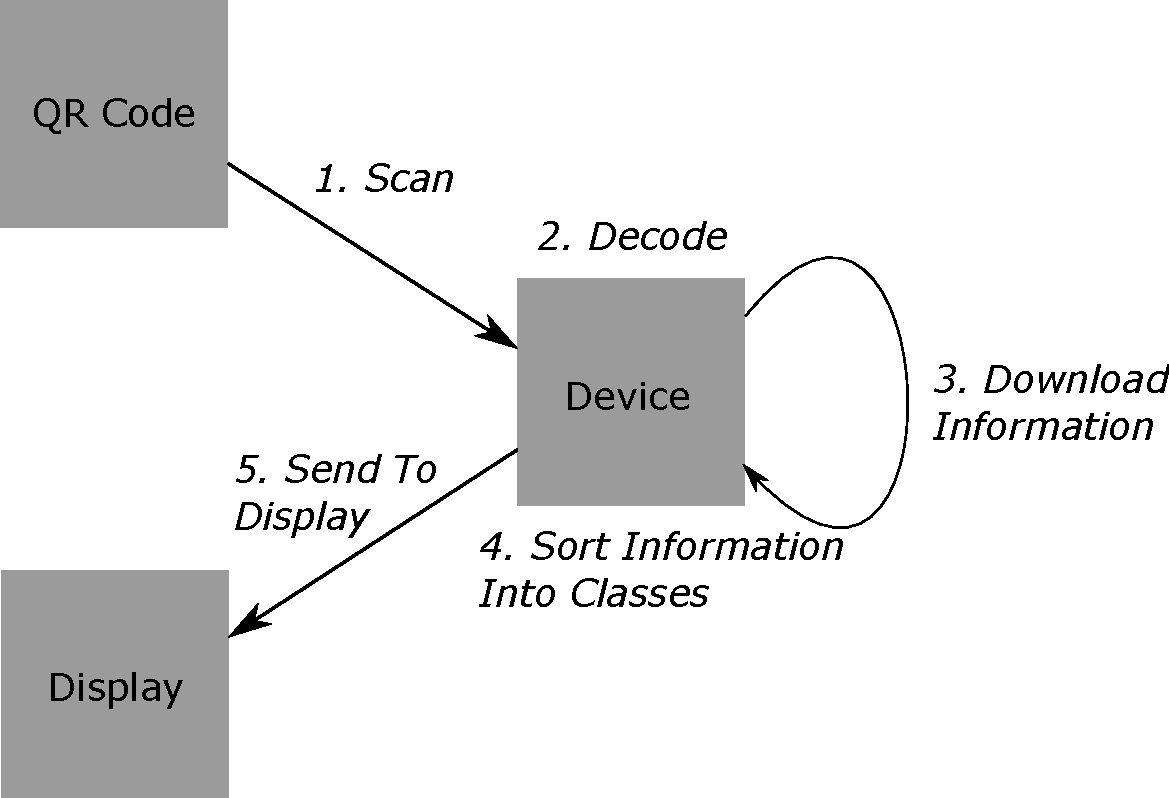
\includegraphics[width=90mm]{images/projectmap4}
		\caption{Application functionality.}
		\label{projectmap}
	\end{figure}

As seen in Figure~\ref{cardDesign}, the application is designed as a slide view, with only one slide being displayed at a time. Instructions are to be divided into several steps, each presented on a separate slide which users may scroll through at their own pace. On Google Glass, users may scroll through the application using voice commands in order to make the application truly hands-free. By applying the slide view design users may focus on one instruction at a time. %Also, the amount of information presented on screen at the same time might also be minimised depending on the limitations of the specific device.
%The application is meant to scan a QR Code, which will give information on the product, enabling the application to retrieve building instructions from a back end database. The instructions, as well as necessary components, will then be presented on screen in a slide show, giving users the ability to scroll through at their own pace.

	\begin{figure}[ht!]
		\centering
		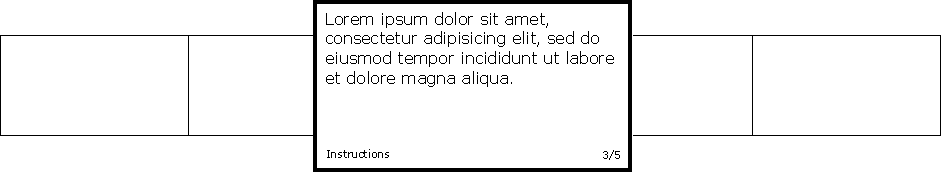
\includegraphics[width=150mm]{images/cardDesign2}
		\caption{A simple sketch of the application's GUI design.}
		\label{cardDesign}
	\end{figure}

The instructions are the major focus of each slide, with each instruction using most of the slide. At the bottom of each slide additional information may be found, such as a label which specifies that the information being presented on the current slide is, for instance, an instruction (other information may also be presented, such as components required to complete the instructions). The design has been heavily inspired by Google's own guidelines~\cite{glassDesignPrinciples} as to how applications for Google Glass should be designed.
%	\begin{figure}[ht!]
%		\centering
%   	\subfloat[The Google Glass application.]{{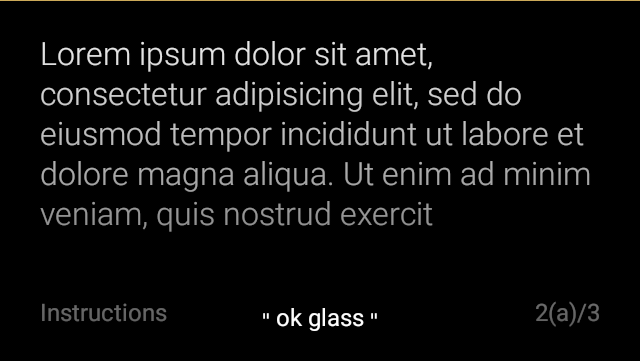
\includegraphics[width=70mm]{images/googleGlassAppScreenshot} }}
%  	 \qquad
%   	\subfloat[The smartphone application.]{{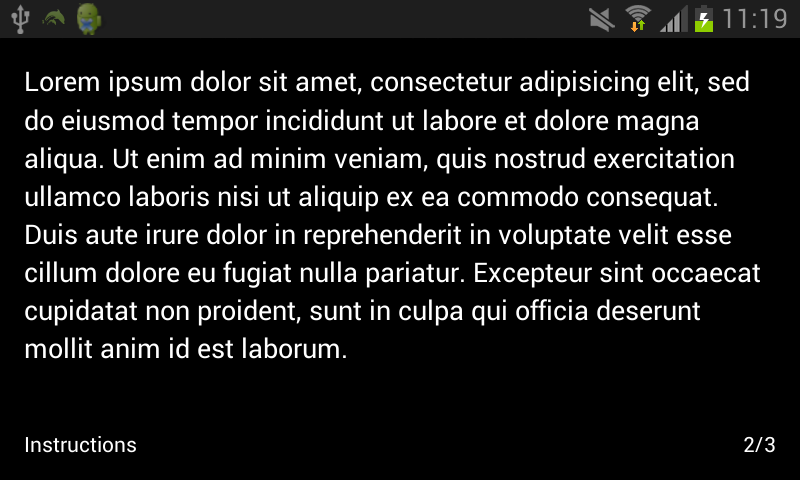
\includegraphics[width=70mm]{images/smartphoneAppScreenshot} }}
%   	\qquad
%		\caption{TODO}
%		\label{applicationScreenshot}
%	\end{figure}

\subsection{Glassware Flow Designer}
Google provides developers with a design tool to help them visualise applications prior to implementation. The design tool, called ``Glassware Flow Designer''~\cite{glasswareFlowDesigner}, allows developers to discover recommended design patterns and to draw out the flow of their application prior to implementation. ``Glassware'' comes from the fact that Google Glass applications are sometimes refered to as ``Glassware''~\cite{glassware}.

In Figure~\ref{glassFlowDesign} the Glass Flow Design for the Google Glass application described in this dissertation is shown. When the application launches the user should scan a QR code. After successfully doing so, the product name will be displayed, in order to help the user confirm that the correct instructions have been downloaded. This is followed by the slides which show the required components. After the list of components follows the instructions. The slides can be controlled either by swiping on the Google Glass touchpad or via voice commands. The next card in line is positioned to the right of the current card.

Although each card could be seen as happening in the future, and should as such be positioned to the left of the current card, it should be noted that the main menu timeline of Google Glass and the application differ in terms of how dependent the cards are of eachother. In the main menu timeline on Google Glass cards are simply related in terms of when they occur. The cards are otherwise not related to each other. In the application, however, each card is dependent on the previous card. The first instruction comes before the second, the second instruction comes before the third, and so forth. As such the cards should be scrolled through more as a story, or a book, where the the user swipes to read the next page.

	\begin{figure}[ht!]
		\centering
		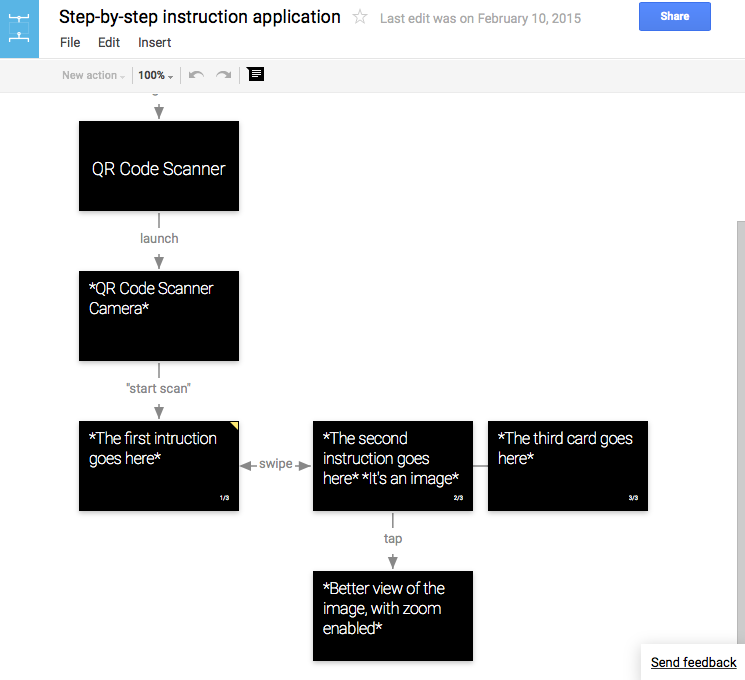
\includegraphics[width=150mm]{images/glaswareFlowDesignerScreenshot}
		\caption{Glass Flow Design of the Google Glass application.}
		\label{glassFlowDesign}
	\end{figure}